\section{Experimental Setup}
\label{expSetup}
The experimental setup that is described in this section, is designed to measure, the properties of LXe scintillation. However it is designed in a modular way, so it can serve different requirements from different future experiments. There are three main building blocks consisting the full setup, The purification and circulation system, the cryogenic system, and the detector system. Each building block can be replaced without effecting the others. The full assembly (figure.~\ref{fig:fulldet}) is held on three separate wracks, one for the DAQ, while the two others which hold the the detector and purification system are joined using a 100mm bar with shock absorbers on both sides.   

\subsection{Gas handling system}
\label{subsec:gas}

A typical LXe detector must keep a high level of purity. Careful selection and meticulously cleaning of all parts before mounting, is needed, however is not sufficient. The desired level of most detectors of impurity concentration is at the level of 1 ppb $O_2$ equivalent~\cite{Aprile:2009dv}. This is crucial to allow ionization electrons drift for several cm. To reach that level in a reasonable amount of time (several days instead of months), continuous purification is needed. The gas system, provides this process, alongside with all gas handling operations such as filling and recuperation.

During purification mode, xenon is taken from the chamber (in liquid phase)
passes through a heat exchanger\footnote{GEA GBS100M-24 plate heat exchanger} where it is heated and vapored. Then the xenon is forced by a KNF diaphragm pump into a hot getter\footnote{MONO-TORR
PS4-MT15-R-2} which cleans the xenon from most impurities. The xenon
also passes through an MKS Mass Flow Controller\footnote{MKS mass flow controller} (MFC). 

After the xenon is purified, it is delivered back to the cryogenic system through the heat exchanger, there the remained xenon gas is liquefied before it continuous back to the chamber. A schematic of this system is shown in fig.~\ref{fig:gasSchematic}.


\begin{figure}[t!]
\centerline{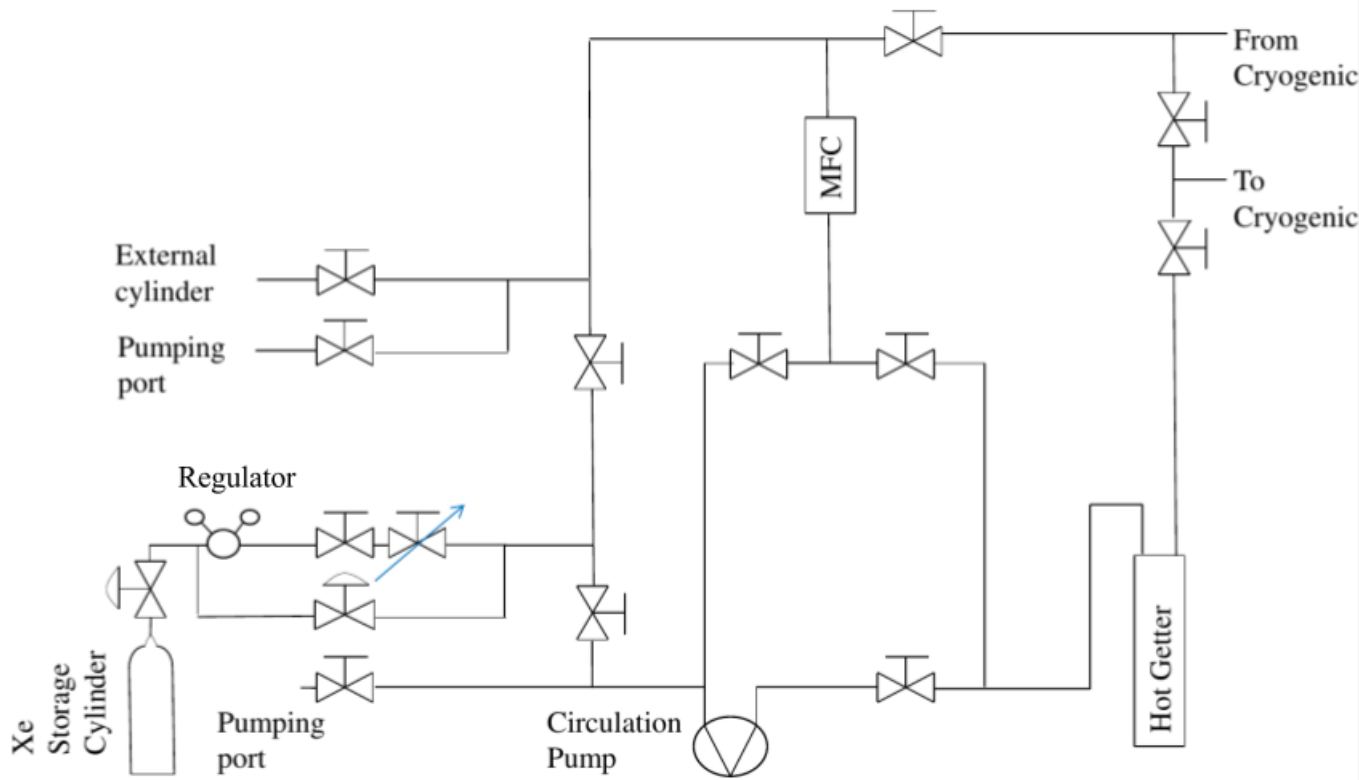
\includegraphics[width=1.\linewidth]{GasSchematics.png}}
\caption{Schematics of the purification system. High presure valves are indicated as valves with arcs. Needle valves are indicated as a valve with an arrow.}
\label{fig:gasSchematic}
\end{figure}
\subsection{Cryogenic System}
\label{subsec:cryo}

Remote cooling is generally used in DM experiments due to background radiating from the cooler to the detector. Although in our system this is not of great importance there are still two advantages to remote cooling, lowering acoustic noise and  flexibility. The cryogenic system is connected on one side to the gas system and on the other to the chamber. Any change in the system (e.g, cryo-cooler type or  model) requires the change of that specific part without changing the detector nor the gas system.

The whole system is made out of super insulated double walls.  The cryo-cooler is connected to the top of the cooling tower and in thermal contact with a copper cold finger. The cold finger design was adopted from XENON1T experiment and is made of large fins for better heat transport from the GXe. The
cryo-cooler of choice is QDrive 20BB 9p6 A 3 AYNBNCO which gives up to 70W
cooling power at LXe temperature. The main advantage of this cooler is that it is thermally regulated, thus there is no need for working at full power and heating to desired temperature, as is done in other xenon experiments.
The gas is liquefied by the fins of the cold finger and the Xe droplets are collected with a funnel and guided by a 1/4" tube to the detector. Evaporated Xe from the detector travels up inside the connecting bellow and gets liquefied again. The xenon that is going out of the cryogenic system towards the hot getter, passes through a heat exchanger, and therefore most of the coming xenon in is already liquefied.

The inner vessel is closed with 6" CF flanges whereas the outer vessel with larger 10" ones. The space between these two vessels is held in vacuum for heat insulation (convection and diffusion). The inner vessel will be covered by multi layer aluminized Myler to prevent heating via radiation.
Initial performance tests, such as leak tests, vacuum condition, cooling and more,were conducted. We are currently liquefying xenon for the first time in a temporary vessel which is the last test before mounting the detector itself.

\subsection{The Detector}
\label{subsec:det}
